\documentclass{beamer}
%Information to be included in the title page:
% Language setting
% Replace `english' with e.g. `spanish' to change the document language
\usepackage[english]{babel}
\usepackage{csquotes}
% Useful packages
\usepackage{amsmath}
\usepackage{graphicx}
\usepackage{hyperref}

\usepackage{biblatex} %Imports biblatex package
\addbibresource{motivation.bib}
\addbibresource{cryo-em.bib}


\title{Intrinsically Disordered Proteins}

\subtitle{Extending the Model of Proteins to Account for Disorder}

\author{Maeve Andersen}


\date{Autumn Semester, 2023}


\begin{document}

\frame{\titlepage}

\begin{frame}
\frametitle{Introduction}
In 1894, Fischer developed a protein model to describe the biological function of proteins. In this model, the protein acts as a key of sorts, where the protein's unique shape determines its unique biological function (the lock) \cite{fischerEinflussConfigurationAuf1894}.
\end{frame}
\begin{frame}
\frametitle{Introduction}
This is the so called "lock and key model" which depends on proteins having rigid 3D structure \cite{fischerEinflussConfigurationAuf1894}.
\end{frame}

\begin{frame}
\frametitle{Introduction}
Today however, protein scientists have found a class of proteins that have no rigid structure, yet play a key role in many biological functions. This class of proteins are called "intrinsically disordered proteins" or proteins having disorder. Disussion of how protein disorder is modeled will be the subject of this talk.
\end{frame}

\begin{frame}
\frametitle{TOC}
[todo insert TOC]
\end{frame}


\begin{frame}
\frametitle{Motivation}
Characterization of disorder in proteins is important as disordered proteins are involved in cellular signaling and regulation,\cite{wrightIntrinsicallyDisorderedProteins2015}
and are associated with human diseases, such as neurodegenerative disease, cardiovascular disease, amyloidoses, cancer, and diabetes.\cite{uverskyIntrinsicallyDisorderedProteins2008}
Although challenging, modern methods of characterizing proteins can provide new insights to crucial protein function human biological mechanisms. \cite{bonomiSimultaneousDeterminationProtein2018}.
\end{frame}

\begin{frame}
\frametitle{Energy Landscapes}
\begin{figure}[h]
    \centering
    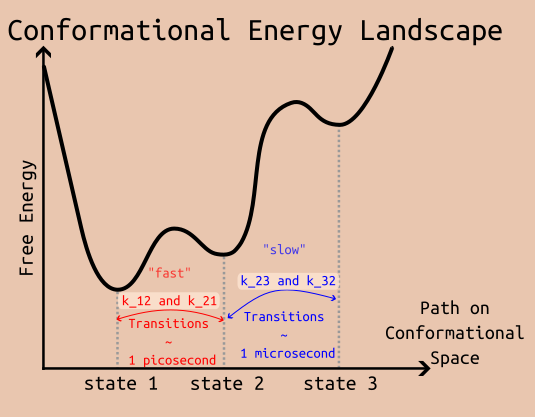
\includegraphics[scale=0.55]{energy-landscape.png}
    \caption{Transition rates and the protein's energy landscape.
        Low populated states often switch "slow" on a time scale of millisecons.
    Highly populated states often switch "fast" on the time scale of picoseconds \cite{bonomiDeterminationProteinStructural2019}. }
    \label{fig:min-bacteria}
\end{figure}
%Transition rates are the kinematics of the protein.
%Dynamics are based on the kinemetics. 

\end{frame}

\begin{frame}
\frametitle{References}
\printbibliography

\end{frame}

\end{document}
